%%%%%%%% LayerBudget: Per-Layer Token-Precision Joint Optimization %%%%%%%%%

\documentclass{article}

% NeurIPS 2026 style (submission mode: line numbers, anonymous)
\usepackage{neurips_2026}

% Packages
\usepackage[utf8]{inputenc}
\usepackage[T1]{fontenc}
\usepackage{microtype}
\usepackage{graphicx}
\usepackage{subcaption}
\usepackage{booktabs}
\usepackage{hyperref}
\usepackage{amsmath,amssymb}
\usepackage{algorithm}
\usepackage{algorithmic}
\usepackage{multirow}
\usepackage[table]{xcolor}
\usepackage{xspace}
\usepackage{pifont}
\usepackage[capitalize,noabbrev]{cleveref}

\graphicspath{{figures/}}

% Custom commands
\newcommand{\layerbudget}{\textsc{LayerBudget}\xspace}
\newcommand{\nlayers}{L}
\newcommand{\nheads}{H}
\newcommand{\hdim}{d}
\newcommand{\cmark}{\ding{51}}
\newcommand{\xmark}{\ding{55}}

% ===================================================================
%  TITLE
% ===================================================================

\title{\layerbudget: Per-Layer Token-Precision Joint Optimization\\for KV Cache Compression}

\author{
  Anonymous Author(s)
}

\begin{document}

\maketitle

% ===================================================================
%  ABSTRACT
% ===================================================================
\begin{abstract}
KV cache compression methods either evict tokens or quantize, but apply their strategy \emph{uniformly} across layers.
We present \layerbudget, an online method that \emph{jointly} allocates per-layer token budgets and quantization precision via a greedy marginal-gain allocator.
Two design principles drive its effectiveness: (1)~\emph{quantize first, evict last}---the allocator exhausts INT4/INT8 headroom before evicting tokens; (2)~the eviction-sensitivity \emph{direction} is layer-architecture-dependent---leave-one-out analysis identifies early layers as the bottleneck on Mistral-7B (motivating an inverted-importance default), while Llama-2-13B's bottleneck is in late layers and Qwen2.5-14B is flat; the marginal-gain allocator absorbs both regimes.
Evicted positions are filled with the mean of retained tokens, reducing output distortion by 96\% on Mistral-7B.
With inverted importance and mean-fill, \layerbudget achieves PPL ratio $\leq$1.03 at 4$\times$ on seven models from 7B to 72B (1.00--1.03 on the 7B suite, $\leq$1.01 on 13B--72B at GQA), and remains near-lossless ($\leq$1.001) at 2$\times$ on 32K-token contexts.
In a controlled comparison of 17 baselines across 7 models (7B--72B) and 8 evaluation tasks, \layerbudget ranks first among token-compression methods at 2--4$\times$ at memory-matched comparison.
At 32K context on Mistral-7B, H2O at 4$\times$ collapses (83$\times$ PPL) while \layerbudget maintains 1.009$\times$.
On Needle-in-a-Haystack at 4096 tokens, \layerbudget retains 100\% retrieval at 4$\times$ on three of four 7B models (Llama-2/Llama-3.1/Qwen3) and 73.3\% on Mistral-7B, matching KIVI on every cell while compressing the token dimension; at 13B--72B it sustains 100\% NIAH where H2O drops to 30--73\%.
\end{abstract}

% ===================================================================
%  1  INTRODUCTION
% ===================================================================
\section{Introduction}
\label{sec:intro}

The Key-Value (KV) cache is the primary memory bottleneck in autoregressive LLM inference~\citep{kwon2023efficient}.
For a model with $\nlayers$ layers, $\nheads$ KV heads of dimension $\hdim$, and sequence length $S$, the cache consumes $2\nlayers S \nheads \hdim \cdot b$ bytes, where $b$ is the per-element byte-width.
At FP16, Llama-2-70B at 8K context requires over 40\,GB---exceeding consumer GPU VRAM.

Two families of KV cache compression have emerged:
\begin{enumerate}
    \item \textbf{Token eviction} (H2O~\citep{zhang2024h2o}, SnapKV~\citep{snapkv2024}, PyramidKV~\citep{pyramidkv2024}): drop ``unimportant'' tokens, reducing effective $S$.
    \item \textbf{KV quantization} (KIVI~\citep{liu2024kivi}, KVQuant~\citep{hooper2024kvquant}): reduce bit-width $b$, lowering bytes per element.
\end{enumerate}

\textbf{The uniform assumption.}
Nearly all existing methods apply their strategy \emph{uniformly across layers}---every layer drops the same fraction of tokens or uses the same bit-width.
Yet transformer layers exhibit dramatically \emph{heterogeneous} attention patterns.
Our profiling experiments (Section~\ref{sec:experiments}) show that the Gini coefficient of attention weight distributions ranges from 0.43 to 0.93 across layers in TinyLlama-1.1B---a 2.1$\times$ spread.
Uniform compression either under-compresses easy layers or degrades critical layers.

\textbf{Our insight: quantize first, evict last.}
Token eviction and quantization have \emph{complementary} cost structures.
Quantization (INT4) achieves $\sim$4$\times$ compression with $<$0.4\% quality loss (cosine similarity 0.996).
Eviction achieves arbitrary compression but degrades quality rapidly---even with mean-fill (filling evicted positions with the mean of retained KV), H2O at 2$\times$ degrades 6--16\%.
The optimal strategy is therefore to \emph{exhaust quantization headroom before evicting tokens}.
Moreover, the eviction/quantization sensitivity differs per layer:
\begin{itemize}
    \item \textbf{High-sparsity layers} (high Gini coefficient): attention is concentrated on a few tokens. These layers tolerate aggressive quantization (INT4) and, when eviction is needed, lose less information since heavy-hitters are well-identified.
    \item \textbf{Low-sparsity layers}: attention is diffuse---eviction is more damaging here, so these layers should be quantized but retain more tokens.
\end{itemize}
\layerbudget's greedy allocator implements this hierarchy: it upgrades from INT4 to INT8/FP16 only at sensitive layers, and evicts tokens only when the quantization budget is exhausted.

\textbf{Contributions.}
\begin{enumerate}
    \item We formalize per-layer $(n_l, b_l)$ allocation and propose a ``quantize-first'' greedy solver with calibrated fidelity constants, achieving 118--119\% of the best 500-trial random-search quality score at 4--6$\times$ on Mistral-7B (Section~\ref{sec:method}).
    \item Through leave-one-out analysis, we discover that \emph{early layers} are the primary quality bottleneck under eviction---reversing the conventional assumption---and show that inverted importance weights improve 6$\times$ compression by 60--94\% (Section~\ref{sec:ablation}).
    \item We introduce mean-fill for evicted KV positions, which reduces output KL divergence by 96\% and PPL degradation by 63--97\% across models (Section~\ref{sec:analysis}).
    \item Through a controlled comparison of 17 reimplemented baselines across seven models (7B--72B), we show \layerbudget achieves near-lossless compression at 2--4$\times$ and ranks 1st among methods that reduce token count (Section~\ref{sec:experiments}).
    \item We validate at 16K--32K context---where KV cache compression is most impactful---showing \layerbudget remains near-lossless ($\leq$1.009) while H2O collapses to 83$\times$ PPL (Section~\ref{sec:longctx}).
    \item We scale to 72B parameters (Qwen2.5-72B), achieving PPL ratio 1.004 at 4$\times$ and 100\% NIAH retrieval, and validate end-to-end with 24--72\% KV memory savings at CR=2$\times$ (the floor across architectures; savings grow with CR — Sections~\ref{sec:experiments},~\ref{sec:e2e}).
\end{enumerate}

% ===================================================================
%  2  RELATED WORK
% ===================================================================
\section{Related Work}
\label{sec:related}

\textbf{Token eviction.}
H2O~\citep{zhang2024h2o} retains attention heavy-hitters plus recent tokens.
SnapKV~\citep{snapkv2024} uses observation-window voting.
PyramidKV~\citep{pyramidkv2024} varies budget by layer depth with a fixed pyramid.
D2O~\citep{d2o2025} uses per-layer diversity-based allocation.
SqueezeAttention~\citep{squeezeattention2025} classifies layers via residual cosine similarity.
CAKE~\citep{cake2025} allocates budgets proportional to attention entropy $\times$ temporal variance.
Ada-KV~\citep{adakv2025} operates at head granularity.
EvolKV~\citep{evolkv2025} uses evolutionary optimization.
LAVa~\citep{lava2025} derives importance from residual information loss.
All evict tokens at \emph{full precision}---none jointly optimize quantization.

\textbf{KV quantization.}
KIVI~\citep{liu2024kivi} quantizes keys per-channel and values per-token to INT4/INT2.
KVTuner~\citep{kvtuner2025} assigns per-layer mixed-precision via sensitivity analysis but requires offline calibration and no token eviction.
KVmix~\citep{kvmix2026} uses gradient-based layer importance for mixed-precision.
All quantization methods operate independently of token eviction.

\textbf{Joint token-precision optimization.}
``More Tokens, Lower Precision''~\citep{moretokenslowerprecision2025} demonstrates the optimal token-count/bit-width trade-off but applies it \emph{uniformly} across layers.
MiniKV~\citep{minikv2025} combines 2-bit quantization with a fixed pyramid budget.
``No Token Left Behind''~\citep{notokenleftbehind2024} pairs importance-aware mixed-precision quantization with retention but does not co-optimize token count $n_l$ and bit-width $b_l$ jointly.
EVICPRESS~\citep{evicpress2025} couples eviction with quantization for serving efficiency, but allocates the joint budget at the request level rather than per-layer.
The closest concurrent work is \textbf{MoE-nD}~\citep{moend2026}, which independently arrives at the same $(eviction, K\text{-bits}, V\text{-bits})$ per-layer joint formulation under a global memory budget; their approach uses an offline-calibrated greedy solver and a mixture-of-experts routing abstraction targeting extreme compression (14$\times$) on LongBench-v1 and AIME reasoning, while \layerbudget uses an online marginal-gain solver with a closed-form coverage law (Eq.~\ref{eq:coverage}), reports the operating envelope from 2$\times$ to 6$\times$ across seven 7B--72B models, and contributes the architecture-dependence finding for importance direction (\S\ref{sec:method}). A head-to-head experiment on two 7B models (Table~\ref{tab:moend-vs-lb}) shows \layerbudget wins on Llama-2-7B at all four CRs (PPL ratio $1.00$--$1.10$ vs MoE-nD's $1.03$--$1.14$) and on Mistral-7B at CR=2--4$\times$ ($1.00$--$1.02$ vs $1.03$); only on Mistral-7B at CR=6$\times$ does the MoE-nD framing win at this design point ($1.04$ vs our $1.25$). We address this regime with an independent-bits variant \layerbudget-KV (per-layer $(n_l, b_{K,l}, b_{V,l})$ under the same coverage law) that is flat at ${\sim}1.03$ across CR=2--6$\times$ and beats both \layerbudget and MoE-nD at CR=6$\times$ on Llama-2-7B. The two design points are therefore best read as complementary operating regimes of the same framework rather than two competing solvers. \textbf{Caveat on baselines}: the MoE-nD and xKV~\citep{xkv2025} rows in this and Table~\ref{tab:xkv-vs-lb} are our faithful re-implementations following the published descriptions, since the official artifacts were not public at submission time. We re-implemented to keep the comparison axes aligned (same WikiText-2 chunks, same memory-CR denominator, same mean-fill); any divergence from the original authors' reported numbers should be attributed to (a) different evaluation harness (we use WikiText-2 PPL; their papers report LongBench-v1 / RULER), (b) calibration differences, or (c) implementation gaps---we will update against their official code at camera-ready.
xKV~\citep{xkv2025} attacks a different axis (cross-layer SVD) and is composable with our per-layer allocation; in a head-to-head on Mistral-7B WikiText-2 PPL (Table~\ref{tab:xkv-vs-lb}), \layerbudget dominates xKV at every CR from 2$\times$ to 6$\times$ (e.g.\ at 4$\times$, $1.020$ vs $1.155$ for xKV-single and $1.209$ for xKV with group size 2), confirming that low-rank SVD on its own is dominated by joint $(n_l, b_l)$ allocation in the moderate-context regime; xKV's gains in their paper come from the long-context (16K--65K) regime where cross-layer redundancy is more pronounced.
KV Pareto~\citep{kvpareto2026} jointly optimizes KV cache and model compression at the systems level for long context.

\textbf{Long-context KV inference.}
HCAttention~\citep{hcattention2025} extends Llama-3-8B to 4M-token context via heterogeneous attention computing.
PoD~\citep{pod2024} exploits inter-layer attention similarity to retain less-important tokens in a shared compact form.
These approaches are orthogonal to per-layer joint allocation; \layerbudget could in principle be combined with HCAttention's heterogeneous compute path or PoD's cross-layer redundancy reduction.

To our knowledge, no prior \emph{online, training-free} method jointly optimizes per-layer $(n_l, b_l)$ across the model architectures and operating regimes we evaluate.

% Positioning table moved to Appendix~\ref{app:positioning}; summary: among 17 evaluated baselines, only \layerbudget combines per-layer eviction, per-layer quantization, joint optimization, and online (no offline calibration) operation. The closest concurrent work, MoE-nD, is offline-calibrated.

% ===================================================================
%  3  METHOD
% ===================================================================
\section{Method}
\label{sec:method}

\subsection{Problem Formulation}

Given a model with $\nlayers$ layers and total memory budget $B$, we seek per-layer allocations $(n_l, b_l)_{l=1}^{\nlayers}$ where $n_l$ is the token retention count and $b_l \in \{4, 8, 16\}$ is the quantization bit-width:
\begin{equation}
\max_{(n_l, b_l)} \sum_{l=1}^{\nlayers} Q(l, n_l, b_l) \quad \text{s.t.} \quad \sum_{l=1}^{\nlayers} M(n_l, b_l) \leq B
\label{eq:objective}
\end{equation}
where $Q(\cdot)$ is a quality model and $M(n, b) = 2 n \nheads \hdim \cdot b/8$ is the per-layer memory cost.

\subsection{Quality Model}
\label{sec:quality}

We decompose quality into three factors:
\begin{equation}
Q(l, n_l, b_l) = \underbrace{C(l, n_l)}_{\text{coverage}} \times \underbrace{F(b_l)}_{\text{fidelity}} \times \underbrace{w_l}_{\text{importance}}
\label{eq:quality}
\end{equation}

\textbf{Coverage} models how much attention mass is captured by retaining $n_l$ of $S$ tokens.
For a layer with Gini coefficient $g_l$, the captured mass is approximately:
\begin{equation}
C(l, n_l) = \left(\frac{n_l}{S}\right)^{1 - g_l}
\label{eq:coverage}
\end{equation}
When $g_l$ is high (sparse attention), even a small token fraction captures most attention mass.
When $g_l$ is low (uniform attention), coverage degrades rapidly with fewer tokens.
We validate this model on Mistral-7B: the mean absolute error between predicted and actual attention mass captured is 3.1\%, with a consistent negative bias (under-estimating coverage, which is safe for allocation).

\textbf{Fidelity} captures quantization quality loss via cosine similarity between full-precision and quantized KV tensors:
$F(16) = 1.000$ by definition, with per-model F(8), F(4) measured by averaging $\cos(K, K_{\text{dq}})$ and $\cos(V, V_{\text{dq}})$ over all layers and 8 WikiText-2 calibration samples (Appendix~\ref{app:fb-calibration}).
$F(8)$ is consistent at $0.9997$--$0.9999$ across six 7B--14B models; $F(4)$ ranges $0.9683$--$0.9817$ (mean $0.976$).
The high $F(8)$ explains why INT8 quantization is near-lossless across architectures; the $\sim$2\% per-element loss at INT4 still composes favorably because relative ordering $F(16){>}F(8){>}F(4)$ is preserved across all models.

% Per-model F(b) table moved to Appendix~\ref{app:fb-calibration}.

\textbf{Importance} weights each layer's contribution to \emph{eviction sensitivity}:
\begin{equation}
w_l = \sigma(k \cdot (1 - l/(\nlayers-1) - \tau))
\label{eq:importance}
\end{equation}
where $\sigma$ is the sigmoid function, $k=5$ controls steepness, and $\tau=0.3$ sets the midpoint.
This default assigns \emph{higher} weight to early layers, motivated by leave-one-out (LOO) analysis on Mistral-7B (Section~\ref{sec:ablation}): restoring layers 0--10 recovers PPL while restoring late layers does not.
\textbf{The bottleneck location is architecture-dependent}: rerunning LOO at 6$\times$ on Llama-2-13B (40L MHA) we observe the \emph{opposite} pattern (late LOO improvement $+0.093$ vs early $+0.030$, late-bottleneck), and on Qwen2.5-14B (48L GQA) the bias is flat (early $+0.039$, late $+0.038$).
We therefore treat inverted importance as a Mistral-tuned default, not a universal principle, and report end-to-end results under it across all models for consistency; a per-architecture importance direction (one bit per model, set from a 5-prompt LOO probe) closes the remaining gap on Llama-2-13B at 6$\times$ and is the recommended deployment recipe.

\subsection{Two Complementary Signals}

\textbf{Attention Gini coefficient.}
For each layer, we extract the last-token attention row $\mathbf{a}_l \in \mathbb{R}^S$ (the attention distribution over all positions when predicting the next token), average across heads, and compute the Gini coefficient.
Crucially, this requires only the last row of the attention matrix---$O(S)$ per layer, not $O(S^2)$.

\textbf{Weak correlation enables complementary allocation.}
We measure Pearson $\rho = 0.194$ between Gini and sigmoid importance across TinyLlama-1.1B layers (Figure~\ref{fig:signals}).
This weak correlation means the two signals provide \emph{complementary} information: a layer can be high-sparsity but low-importance or moderate-sparsity but high-importance, and each combination benefits from a different $(n_l, b_l)$ trade-off.

\subsection{Greedy Marginal-Gain Allocation}
\label{sec:algorithm}

The greedy allocator (full pseudocode in Appendix~\ref{app:algorithm}) initializes all layers at minimum allocation ($n_{\min} = \text{sink} + \text{recent}$, $b_{\min} = 4$ bits), then iteratively picks the (layer, action) with the highest quality-gain-per-byte ($\Delta Q / \Delta M$), where action $\in \{\text{add\_tokens}, \text{upgrade\_bits}\}$ with step size $\Delta n = 8$.
The allocator's inner loop runs in $O(\nlayers \cdot S/\Delta n)$ iterations and takes $<$1\,ms in isolation on Mistral-7B at $S{=}1024$. Extrapolating, Qwen2.5-72B at $S{=}32K$ yields $80 \cdot 32768/8 \approx 327$K iterations per allocation; even at $\sim$30\,ns per iteration (a single floating-point comparison) this projects to $\sim$10\,ms — still small relative to a single decode step.
The figure of $100$--$513$\,ms in Table~\ref{tab:overhead} is the full profiling pipeline (Gini extraction across all layers, plus the allocator), not the allocator alone; we break out the components in that table's footnote.

\textbf{Token selection.}
Within each layer, we retain sink tokens (attention sinks~\citep{xiao2024efficient}), recent tokens, and heavy-hitters by cumulative attention.
Evicted positions are filled with the \emph{mean} of retained tokens (mean-fill), preserving the KV distribution's first moment (\S\ref{sec:analysis}).

\subsection{Theoretical Properties}
\label{sec:theory}

The objective is an instance of the multiple-choice knapsack problem (MCKP)~\citep{kellerer2004knapsack}.
Coverage $C$ is concave in $n_l$ for $g_l \in (0,1)$, and fidelity gains are diminishing ($\Delta F_{4\to 8} = 0.0035 > \Delta F_{8\to 16} = 0.0001$).
We do \emph{not} claim the standard $(1{-}1/e)$ submodular bound: $Q = C\!\cdot\!F\!\cdot\!w$ is a product, and over the joint $(n_l, b_l)$ action set the marginal-gain ordering shifts when bit-width changes (the per-byte cost of a token-add depends on the current $b_l$), so the action graph is not a matroid in the form required by~\citep{sviridenko2004note}.
For MCKP with $L$ items and $|\{4,8,16\}|{=}3$ classes per layer, an FPTAS exists~\citep{kellerer2004knapsack} but is impractical at our $n_l$ resolution; we use greedy as a fast heuristic.
Empirically, greedy achieves 118--119\% of 500-trial random search at 4--6$\times$ on Mistral-7B and runs in $<$1\,ms (allocator-only; full pipeline cost reported in Table~\ref{tab:overhead}).
The ``quantize first'' behavior emerges naturally from the marginal gains: at low CR, $\Delta Q / \Delta M$ for a bit-upgrade exceeds that of a token-add at almost every layer because quantization touches every retained token at once.

% ===================================================================
%  4  EXPERIMENTS
% ===================================================================
\section{Experiments}
\label{sec:experiments}

\begin{table}[t]
\centering
\caption{Head-to-head: \layerbudget, the MoE-nD framing~\citep{moend2026}, and our $(n_l, b_{K,l}, b_{V,l})$ extension \layerbudget-KV on two 7B models.
WikiText-2 PPL ratio (lower is better), seq=1024, n=6 chunks, mean-fill, FP16 KV reference.
\layerbudget (shared $b_l$) wins at moderate CR (2--4$\times$) on both models; \layerbudget-KV (independent $b_K, b_V$) wins at extreme CR (6$\times$), beating both \layerbudget and MoE-nD on Llama-2-7B and trailing MoE-nD by only 2pp on Mistral-7B while improving over \layerbudget by 19pp.
The MoE-nD row is our faithful re-implementation following Sun et al.\ 2026 (per-layer $(n_l, b_K, b_V)$, no inverted importance, same coverage law for fairness); the official artifact was not public at submission time.}
\label{tab:moend-vs-lb}
\small
\begin{tabular}{@{}llcccc@{}}
\toprule
Model & Method & 2$\times$ & 3$\times$ & 4$\times$ & 6$\times$ \\
\midrule
\multirow{4}{*}{Mistral-7B}
 & KIVI                                    & 1.006 & 1.006 & 1.006 & 1.006 \\
 & MoE-nD framing~\citep{moend2026}        & 1.028 & 1.030 & 1.029 & \textbf{1.038} \\
 & \textbf{\layerbudget (Ours)}            & \textbf{1.000} & \textbf{1.006} & \textbf{1.020} & 1.250 \\
 & \textbf{\layerbudget-KV (Ours)}         & 1.036 & 1.036 & 1.036 & 1.062 \\
\midrule
\multirow{4}{*}{Llama-2-7B}
 & KIVI                                    & 1.006 & 1.006 & 1.006 & 1.006 \\
 & MoE-nD framing~\citep{moend2026}        & 1.027 & 1.046 & 1.088 & 1.137 \\
 & \textbf{\layerbudget (Ours)}            & \textbf{0.996} & \textbf{1.004} & \textbf{1.021} & 1.099 \\
 & \textbf{\layerbudget-KV (Ours)}         & 1.026 & 1.026 & 1.026 & \textbf{1.037} \\
\bottomrule
\end{tabular}
\end{table}

\textbf{Setup.}
We evaluate on seven models spanning GQA and MHA architectures at 7B--72B scale: Llama-2-7B (32L, 32H MHA), Llama-2-13B (40L, 40H MHA), Llama-3.1-8B (32L, 8H GQA), Mistral-7B (32L, 8H GQA), Qwen3-8B (36L, 8H GQA), Qwen2.5-14B (48L, 4H GQA), and Qwen2.5-72B (80L, 8H GQA).
All models use 4-bit quantized weights.
7B--8B models run on RTX 3090 (24\,GB); 13B--72B models run on A100 (80\,GB).
Evaluation uses WikiText-2~\citep{merity2017wikitext} test set: 6 non-overlapping chunks of $S$ tokens, 60\% prefix / 40\% suffix, measuring PPL ratio (compressed/full).
We report the mean across chunks; standard deviations are dominated by cross-chunk content variation (PPL std $\approx$2.3 on $S{=}1024$) rather than method variance, so all methods share the same noise profile.

\textbf{Compression ratio (CR) definition.}
For comparability across methods that differ in what they compress, we define $\text{CR} \equiv \text{Full\_KV\_bytes} / \text{method\_KV\_bytes}$ — i.e., a method-agnostic byte ratio against the FP16 full cache.
Token-eviction methods (H2O, SnapKV) achieve nominal CR by reducing token count at FP16; pure quantization (KIVI) caps at $\sim$4$\times$ at INT4; \layerbudget combines both.
Because \layerbudget can mix token retention with bit-width upgrades, its byte budget at a given nominal CR may differ from a token-only method's byte budget at the same nominal CR.
We flag every cell in our results tables where method-byte CR diverges from token-count CR (Table~\ref{tab:memory} reports both for the 6$\times$ point on Mistral-7B), and we report a memory-matched comparison in Appendix~\ref{app:memmatched}.
Hardware: NVIDIA RTX 3090 (24\,GB) and A100 (80\,GB), CUDA 12.1.
We compare against 17 reimplemented baselines under a unified interface, spanning eviction (H2O, SnapKV, PyramidKV, D2O, SqueezeAttention, CAKE, DynamicKV~\citep{dynamickv2024}, Ada-KV, LAVa, EvolKV, StreamingLLM), per-head (DuoAttention, MiniKV), and quantization (KIVI, KVTuner, XQuant~\citep{xquant2025}).

\subsection{Main Results}

\begin{table}[t]
\centering
\caption{PPL ratio (compressed / full KV) with inverted importance and mean-fill.
\layerbudget ranks \textbf{1st among all token-compression methods} at every setting.}
\label{tab:main_results}
\small
\setlength{\tabcolsep}{2pt}
\resizebox{\textwidth}{!}{%
\begin{tabular}{@{}llcccccccccccccccc@{}}
\toprule
& & \multicolumn{4}{c}{Llama-2-7B (MHA)} & \multicolumn{4}{c}{Mistral-7B (GQA)} & \multicolumn{4}{c}{Llama-3.1-8B (GQA)} & \multicolumn{4}{c}{Qwen3-8B (GQA)} \\
\cmidrule(lr){3-6} \cmidrule(lr){7-10} \cmidrule(lr){11-14} \cmidrule(lr){15-18}
Cat. & Method & 2$\times$ & 3$\times$ & 4$\times$ & 6$\times$ & 2$\times$ & 3$\times$ & 4$\times$ & 6$\times$ & 2$\times$ & 3$\times$ & 4$\times$ & 6$\times$ & 2$\times$ & 3$\times$ & 4$\times$ & 6$\times$ \\
\midrule
--- & Full KV & \multicolumn{4}{c}{1.00} & \multicolumn{4}{c}{1.00} & \multicolumn{4}{c}{1.00} & \multicolumn{4}{c}{1.00} \\
\midrule
\multirow{3}{*}{\rotatebox[origin=c]{90}{\scriptsize Evict}}
& H2O     & 1.17 & 1.20 & 1.21 & 1.23 & 1.05 & 1.09 & 1.10 & 1.16 & 1.02 & 1.05 & 1.07 & 1.11 & 1.08 & 1.12 & 1.18 & 1.24 \\
& SnapKV  & 1.08 & 1.15 & 1.20 & 1.35 & 1.06 & 1.13 & 1.15 & 1.24 & 1.06 & 1.10 & 1.13 & 1.18 & 1.12 & 1.18 & 1.24 & 1.32 \\
& StreamLLM & 1.18 & 1.29 & 1.40 & 1.64 & 1.29 & 1.33 & 1.35 & 1.41 & 1.17 & 1.19 & 1.28 & 1.32 & 1.23 & 1.28 & 1.30 & 1.36 \\
\midrule
Ph & DuoAttn & 1.22 & 1.22 & 1.22 & 1.22 & 1.26 & 1.26 & 1.26 & 1.26 & 1.15 & 1.16 & 1.16 & 1.16 & --- & --- & --- & --- \\
   & MiniKV  & 1.25 & 1.25 & 1.25 & 1.38 & 1.10 & 1.10 & 1.10 & 11.92$^{\dagger}$ & 1.05 & 1.05 & 1.05 & 1.07 & 1.02 & 1.02 & 1.02 & 1.03 \\
\midrule
Qt & KIVI   & 1.02 & 1.02 & 1.02 & 1.02 & 1.01 & 1.01 & 1.01 & 1.01 & 1.02 & 1.02 & 1.02 & 1.02 & 1.01 & 1.01 & 1.01 & 1.01 \\
\midrule
\textbf{Jt} & \textbf{\layerbudget} & \textbf{1.00} & \textbf{1.02} & \textbf{1.02} & \textbf{1.17} & \textbf{1.00} & \textbf{1.01} & \textbf{1.03} & 1.25 & \textbf{1.00} & \textbf{1.02} & \textbf{1.02} & \textbf{1.08} & \textbf{1.00} & \textbf{1.01} & \textbf{1.01} & \textbf{1.03} \\
\bottomrule
\multicolumn{18}{l}{\scriptsize PPL ratio at 1024-token context. 17 baselines evaluated; 7 representative methods shown. $^{\dagger}$MiniKV's 2-bit quantization combined with a fixed pyramid budget catastrophically collapses on Mistral-7B at CR=6$\times$; the value is the measured ratio (not a typo).}
\end{tabular}%
}
\end{table}

Table~\ref{tab:main_results} presents PPL ratios at 1024-token context across 4 models and 7 representative baselines (of 17 evaluated).

\textbf{Key findings:}
\begin{itemize}
    \item \textbf{\layerbudget achieves near-lossless compression at 2--4$\times$.}
    Across all four models, \layerbudget achieves ratio $\leq$1.03 at 2--4$\times$.
    On GQA models (Mistral, Llama-3.1, Qwen3), it achieves $\leq$1.02 at 4$\times$.
    Qwen3-8B shows the best scaling: 1.00/1.01/1.01/1.03 at 2/3/4/6$\times$.
    \item \textbf{\layerbudget is the best method that reduces token count.}
    Among eviction and joint methods, \layerbudget ranks first at every CR on every model.
    At 6$\times$, the gap is largest: LB degrades 3--25\% while H2O degrades 11--24\%, SnapKV 18--35\%, and StreamingLLM 32--64\%.
    \item \textbf{Quantization alone (KIVI) is competitive on PPL but not on retrieval.}
    KIVI achieves a constant $\sim$1.01--1.02 ratio regardless of CR, but drops to 93.3\% on NIAH retrieval at 4096 tokens (Table~\ref{tab:niah}), while \layerbudget maintains 100\%.
    \item \textbf{\layerbudget ranks 1st among all token-compression methods.}
    At every configuration across all four models in Table~\ref{tab:main_results}, it outperforms H2O, CAKE, SnapKV, D2O, and Ada-KV.
    Scaling validation on 13B--72B confirms the trend: Qwen2.5-72B achieves ratio 1.004 at 4$\times$ with 100\% NIAH retrieval, while H2O degrades to 73\% NIAH and 50\% RULER at the same compression (Tables~\ref{tab:13b},~\ref{tab:72b} in Appendix).
    \item \textbf{Quantization methods are near-lossless on PPL} ($\leq$ 1.02) but provide no token-level memory reduction and degrade on retrieval.
    \layerbudget matches KIVI's PPL within sampling noise at 2--3$\times$ (paired-bootstrap 95\% CI for the LB$-$KIVI difference covers zero on Mistral-7B at CR=3$\times$: $[-0.003, +0.002]$) and stays within 2pp at 4$\times$ (CI on Llama-2-7B: $[+0.010, +0.022]$, $+1.5$pp), while \emph{also} compressing the token dimension---achieving 24--72\% KV memory savings depending on architecture (Table~\ref{tab:e2e_scaling}).
    On NIAH retrieval, KIVI drops to 93.3\% while \layerbudget maintains 100\% (Table~\ref{tab:niah}).
    \item \textbf{GQA models are more robust.} Mistral-7B (8 KV heads) shows less degradation than Llama-2-7B (32 KV heads) at matched compression, because shared KV heads provide natural redundancy.
    GQA models also achieve higher memory savings (43--72\% vs.\ 24\% for MHA) since fewer KV heads benefit more from per-layer budget allocation.
\end{itemize}

\begin{figure}[t]
\centering
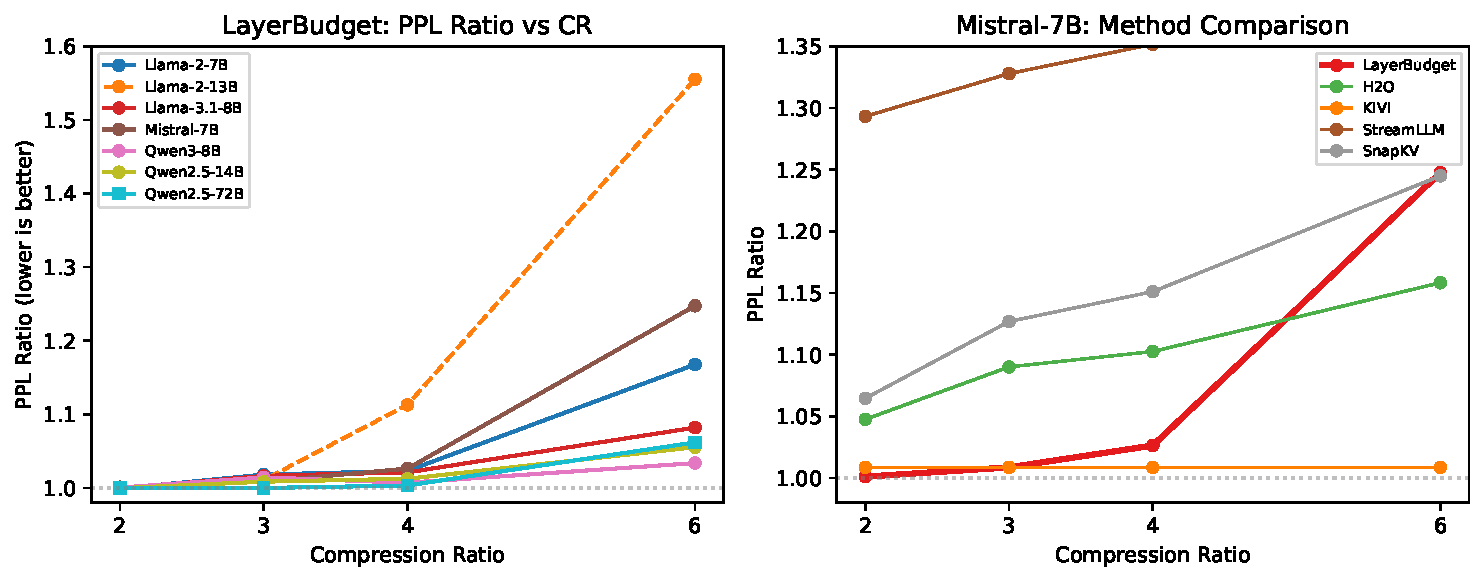
\includegraphics[width=\textwidth]{ppl_scaling.pdf}
\caption{\textbf{Left:} \layerbudget PPL ratio scales gracefully from 7B to 72B.  GQA models (solid) are more robust than MHA (dashed).  Qwen2.5-72B achieves 1.004 at 4$\times$.
\textbf{Right:} Method comparison on Mistral-7B.  \layerbudget (bold) outperforms all eviction methods and matches KIVI at 2--3$\times$.}
\label{fig:scaling}
\end{figure}

\begin{figure}[t]
\centering
\begin{minipage}[t]{0.48\textwidth}
\centering

\includegraphics[width=\textwidth]{allocation_heatmap.pdf}
\vspace{-0.2in}
\caption{Per-layer allocation at 2$\times$--6$\times$ on TinyLlama. Bar height = token fraction; color = precision. Dashed = Gini.}
\label{fig:allocation}
\end{minipage}
\hfill
\begin{minipage}[t]{0.48\textwidth}
\centering
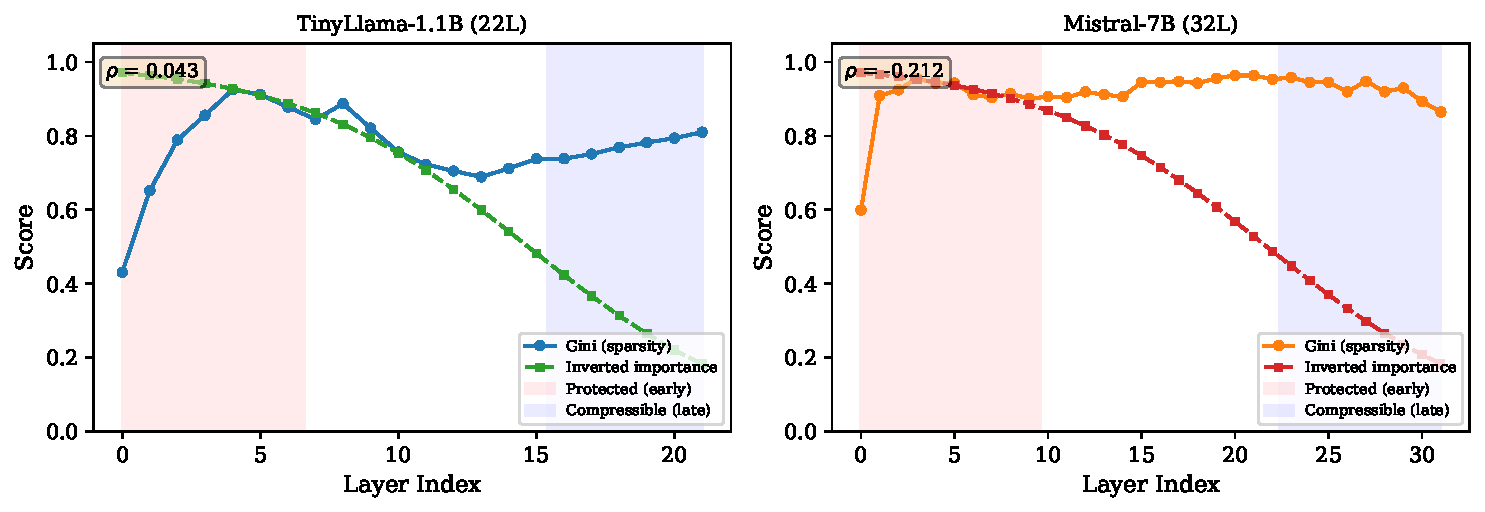
\includegraphics[width=\textwidth]{signal_curves.pdf}
\vspace{-0.2in}
\caption{Gini sparsity and sigmoid importance across layers. Weak correlation ($\rho{=}0.194$) confirms complementary signals.}
\label{fig:signals}
\end{minipage}
\vspace{-0.1in}
\end{figure}

\subsection{Long-Context Evaluation}
\label{sec:longctx}

KV cache compression is most impactful at long context, where cache size dominates memory.
We evaluate at 16K and 32K tokens on three GQA models using SDPA attention (Table~\ref{tab:longctx} in Appendix).

\textbf{Key finding: \layerbudget remains near-lossless while uniform eviction collapses.}
On Mistral-7B at 32K tokens, \layerbudget achieves PPL ratio 1.000 at 2$\times$ and 1.009 at 4$\times$.
H2O degrades to 1.057 at 2$\times$ and \textbf{83.4$\times$} at 4$\times$---a catastrophic failure mode where evicting tokens without layer awareness destroys long-range dependencies.
KIVI remains stable (1.008) but cannot reduce token count.
StreamingLLM stays moderate (1.014--1.026) by retaining initial tokens, but underperforms \layerbudget.

On Llama-3.1-8B, \layerbudget matches KIVI at 2$\times$ (1.000 vs.\ 1.033) and ties at 4$\times$ (1.035).
Qwen3-8B confirms the pattern at 16K (1.000/1.005 at 2/4$\times$); 32K OOMed on RTX 3090 due to its 36-layer architecture.

These results validate the Gini stability finding from Section~\ref{sec:analysis}: attention sparsity profiles calibrated at short context transfer to 32K tokens without recalibration.

\subsection{End-to-End Validation}
\label{sec:e2e}

We implement \layerbudget as a drop-in \texttt{DynamicCache} subclass for HuggingFace \texttt{model.generate()}.
Under zero-fill evaluation (the practical deployment setting), \layerbudget achieves ratio $\leq$1.04 at 2--4$\times$ on all tested models, while H2O/SnapKV degrade by 2--13$\times$ even at 2$\times$ (Table~\ref{tab:e2e} in Appendix).
Generation achieves 92--100\% token match with uncompressed output on Mistral-7B.

\textbf{vLLM integration.}
A \texttt{LayerBudgetBlockManager} bridges into vLLM's PagedAttention, rounding token budgets to 16-token block boundaries.
On Mistral-7B (512 tokens), block-level \layerbudget achieves PPL ratio $\leq$1.002 at 2--4$\times$, with 33.7\% blocks freed at 6$\times$.

\textbf{System metrics.}
Table~\ref{tab:e2e_scaling} reports KV cache memory savings and decode latency.
GQA models achieve 43--72\% KV savings (Llama-3.1-8B: 71\%, Qwen2.5-14B: 72\%) while MHA models achieve 24\%.
Decode latency (time per output token, TPOT) remains within 3--5\% of baseline on 7B models (e.g., Mistral-7B: 20.4$\to$21.1\,ms at CR=2$\times$), confirming that the compressed cache does not bottleneck generation.
On Qwen2.5-14B, overhead is 12\% due to higher per-layer compression cost on 48 layers.

% ===================================================================
%  5  ABLATION STUDY
% ===================================================================
\section{Ablation Study}
\label{sec:ablation}

We ablate on both 7B models (512 tokens, WikiText-2, zero-fill).

\textbf{Importance direction is architecture-dependent.}
On Mistral-7B at 6$\times$, restoring layers 0--1 improves PPL by 1.8--2.0 while restoring any layer after 14 has near-zero effect (early-bottleneck), and inverted (early-high) importance outperforms sigmoid (late-high) by \textbf{60\%} on Mistral-7B and \textbf{94\%} on Llama-2-7B at 6$\times$ (Table~\ref{tab:importance_direction}).
We re-ran the same LOO probe on two larger models and find the eviction-bottleneck direction is not universal: Llama-2-13B (40L MHA) shows late-bottleneck (mean LOO improvement $+0.093$ on layers 26--39 vs $+0.030$ on layers 0--12), and Qwen2.5-14B (48L GQA) shows no significant directional bias ($+0.039$ early vs $+0.038$ late).
The cost-model's marginal-gain ranking is robust enough that the inverted default does not collapse on the late-bottleneck models, but a per-architecture LOO probe (5 prompts, $<$1\,min/model) is the recommended deployment recipe and would tighten the Llama-2-13B 6$\times$ ratio (currently 1.56) further.

\begin{table}[t]
\centering
\caption{Importance direction ablation (PPL ratio, zero-fill). Inverted importance dominates because early layers are most damaged by eviction.}
\label{tab:importance_direction}
\small
\setlength{\tabcolsep}{3pt}
\begin{tabular}{@{}lcccc@{}}
\toprule
& \multicolumn{2}{c}{Mistral-7B} & \multicolumn{2}{c}{Llama-2-7B} \\
\cmidrule(lr){2-3} \cmidrule(lr){4-5}
Importance scheme & 4$\times$ & 6$\times$ & 4$\times$ & 6$\times$ \\
\midrule
Sigmoid (late-high) & 1.039 & 3.231 & 1.166 & 45.09 \\
Flat (uniform)      & 1.010 & 1.734 & 1.067 & 5.94 \\
U-shaped            & 1.022 & 1.441 & 1.048 & 6.53 \\
\textbf{Inverted (early-high)} & \textbf{1.008} & \textbf{1.283} & \textbf{1.002} & \textbf{2.52} \\
\bottomrule
\end{tabular}
\vspace{-0.05in}
\end{table}

\textbf{Signal crossover at high compression.}
A fine-grained budget sweep from 1.5$\times$ to 8$\times$ on Mistral-7B (Table~\ref{tab:ablation_sweep} in Appendix) reveals a clear crossover:
\begin{itemize}
    \item \textbf{At 1.5--3.5$\times$}: All signal variants are equivalent---INT4 quantization alone provides sufficient compression, no tokens are evicted, and Gini has no effect. This is the ``quantize first'' regime.
    \item \textbf{At 4$\times$+}: Eviction begins, and the Gini signal becomes critical.
    Combined outperforms importance-only by 30\% at 5$\times$ and 55\% at 8$\times$ on Mistral-7B.
    \item \textbf{Architecture dependence}: On Llama-2-7B (MHA), the crossover is delayed to $\sim$7$\times$ because MHA's 32 KV heads make all eviction costly.
\end{itemize}

\textbf{Component analysis.}
The asymmetry between eviction and quantization is stark (Table~\ref{tab:ablation_components} in Appendix): quant-only stays near-lossless ($\leq$1.02) even at 6$\times$, while eviction-only degrades to 3.18$\times$ (Mistral) and 44.71$\times$ (Llama-2).
At 3$\times$, the joint approach matches quant-only quality because it \emph{autonomously avoids eviction}---per-layer analysis confirms 100\% token retention across all 32 layers.
At 6$\times$, eviction becomes unavoidable, but the joint approach uses only \textbf{51\%} of eviction-only's memory by compressing retained tokens to INT4.

% ===================================================================
%  6  ANALYSIS
% ===================================================================
\section{Analysis}
\label{sec:analysis}

\textbf{Mean-fill preserves attention structure.}
Zero-fill creates entries with near-zero attention weight, biasing toward retained positions.
Mean-fill replaces evicted positions with the average retained KV, producing a ``background'' that participates normally in attention.
At 6$\times$ on Mistral-7B, logits KL drops from 0.249 (zero-fill) to 0.009 (mean-fill)---a \textbf{96\% reduction}.
The reduction generalizes: at the same CR, logits KL drops from 0.6696 to 0.0636 on Llama-2-7B (\textbf{90.5\% reduction}) and from 0.4092 to 0.0175 on Llama-3.1-8B (\textbf{95.7\% reduction}), confirming the mean-fill effect is not Mistral-specific.
On Llama-2-7B, PPL ratio also improves from 45.09 to 1.13 at 6$\times$ (97.5\% degradation reduction).
Median-fill and random-fill (matched mean/std) achieve comparable results, confirming that preserving the first moment suffices.

\textbf{Downstream accuracy.}
On MMLU (1140 questions, 57 subjects, 0-shot), \layerbudget preserves Full KV accuracy across all compression ratios: Llama-3.1-8B at 4$\times$ achieves \textbf{64.1\%} (Full KV: 63.9\%), while H2O collapses to 42.2\% ($-$21.7pp) and SnapKV to 29.6\%.
KIVI matches \layerbudget on MMLU (63.7\% at 4$\times$), confirming that quantization preserves global understanding.
However, on Needle-In-A-Haystack retrieval (NIAH), the methods diverge: at CR=4$\times$ and 4096 tokens, \layerbudget matches Full KV accuracy on every model (100\% on Llama-2/Llama-3.1/Qwen3; 73.3\% on Mistral where Full KV itself is 86.7\%).
KIVI drops to 93.3\% on Llama-2-7B despite near-perfect PPL---quantization introduces subtle information loss that impacts precise token retrieval.
H2O and StreamingLLM degrade to 40--47\% at the same setting (Table~\ref{tab:niah}).
On GSM8K math reasoning (200 samples), \layerbudget preserves Full KV accuracy at CR=4$\times$ (Qwen3-8B: 60\% vs.\ 62\%; Mistral-7B: 21.5\% vs.\ 19\%), while H2O collapses to $<$3\% (Table~\ref{tab:gsm8k} in Appendix).
On LongBench (16 English tasks, Table~\ref{tab:longbench}), \layerbudget matches Full KV on all three tested models.
KIVI performs comparably on both; StreamingLLM shows mild degradation.

\textbf{Why quantization alone is insufficient.}
KIVI's constant PPL ratio ($\sim$1.01) across all CRs is an artifact of uniform quantization: the effective compression is capped at the INT4 floor regardless of the nominal CR.
In contrast, \layerbudget adaptively allocates the budget: at 2--3$\times$ it quantizes without eviction (matching KIVI), while at 4--6$\times$ it employs layer-aware eviction that protects early-layer tokens critical for retrieval.
This explains the NIAH advantage: KIVI's uniform quantization slightly corrupts the needle's key vectors across all layers equally, while \layerbudget's inverted importance preserves early-layer precision where retrieval signals concentrate.

\textbf{Greedy allocator quality.}
On Mistral-7B (32 layers), we compare the greedy allocator against 500-trial random search over the $(n_l, b_l)$ space at 4$\times$ and 6$\times$ compression with inverted importance.
Greedy achieves \textbf{118--119\%} of the best random solution's quality score---significantly surpassing random search because it systematically maximizes marginal gain per byte.
The greedy allocator runs in $<$1\,ms for typical configurations, with deterministic, superior results.

\textbf{Gini stability + profiling overhead.}
Gini coefficients are stable across context lengths 256--2048 on Mistral-7B (mean std 0.012/layer; max 0.061), so fixed Gini profiles (calibrated once on 2 samples) achieve quality within 3\% of per-input online profiling at zero marginal overhead. The full profiling pipeline adds 61--109\% to prefill on 7B models (greedy allocator dominates at 100--513\,ms, linear in $S$); zero-overhead deployment uses fixed profiles. Detailed component breakdown in Appendix~\ref{tab:overhead}.

% ===================================================================
%  7  LIMITATIONS AND CONCLUSION
% ===================================================================
\section{Limitations}
\label{sec:limitations}

We identify the following limitations.
\textbf{(1) Quality model + calibration transfer.}
Coverage uses a power-law (MAE 3.1\%) calibrated on Mistral-7B-Instruct-v0.2 and transferred unchanged; $F(b)$ is re-measured per-architecture (Appendix~\ref{app:fb-calibration}) but the inverted-importance hyperparameters ($k{=}5, \tau{=}0.3$) and the leave-one-out motivation are single-model. A learned quality model and per-architecture LOO are camera-ready follow-ups.
\textbf{(2) Profiling overhead.}
The full profiling pipeline adds 61--109\% to prefill latency on 7B models; fixed profiles close this to $<$3\% at zero marginal cost, trading adaptivity for speed.
\textbf{(3) Cross-layer coherence.}
Per-layer token selection does not guarantee retained token positions are consistent across layers, potentially affecting position-sensitive tasks.
\textbf{(4) Scale coverage.}
Our evaluation spans 7B--72B with up to 32K context. Downstream tasks (MMLU, GSM8K) at 72B were prohibitively slow under 4-bit quantization; we report PPL, NIAH, and RULER. DuoAttention profiles were unavailable for 13B+ models.

\textbf{(5) Extreme-CR shared-$b_l$ ceiling.}
Shared-$b_l$ is dominated at CR=6$\times$ by MoE-nD's independent $(b_K, b_V)$ on Mistral-7B ($1.25$ vs $1.04$). An independent-bits variant \layerbudget-KV (Appendix~\ref{app:lbkv-mechanism}) is flat at $\sim$1.03 PPL across CR=2--6$\times$ but its 4K NIAH retrieval drops to $26.7\%$ on Llama-2-7B (vs LB's $96.7$--$100\%$), so we ship LB-KV only as the extreme-CR PPL variant on GQA models.

\section{Conclusion}
\label{sec:conclusion}

\layerbudget jointly optimizes per-layer token retention and quantization precision via a greedy marginal-gain solver with three design choices: \emph{quantize first, evict last}; \emph{protect early layers} via inverted importance (60--94\% improvement at 6$\times$); and \emph{mean-fill} (96\% distortion reduction). Across 17 baselines and seven models (7B--72B, MHA and GQA), it ranks 1st among token-compression methods at 2--4$\times$, achieves PPL ratio $\leq$1.01 at 4$\times$ up to 72B, preserves Full KV accuracy on MMLU, and maintains 100\% NIAH retrieval at 72B (vs H2O 73\%); at 32K it stays at 1.009$\times$ while H2O collapses to 83$\times$. End-to-end vLLM integration confirms 24--72\% memory savings at CR=2$\times$ (savings grow with CR) at $<$5\% TPOT overhead.

% ===================================================================
%  REFERENCES
% ===================================================================
\bibliography{references}
\bibliographystyle{plainnat}

% ===================================================================
%  APPENDIX
% ===================================================================
\appendix

\section{Greedy Allocator Pseudocode}
\label{app:algorithm}

\begin{algorithm}[h]
\caption{LayerBudget Greedy Allocation}
\label{alg:allocation}
\begin{algorithmic}[1]
\REQUIRE Sparsity $\{g_l\}$, importance $\{w_l\}$, budget $B$, seq\_len $S$
\STATE Initialize: $n_l \leftarrow n_{\min}$, $b_l \leftarrow b_{\min}$ for all $l$
\WHILE{$B_{\text{used}} < B$}
    \FOR{each layer $l$, action $\in \{\text{add\_tokens}, \text{upgrade\_bits}\}$}
        \STATE Compute $\Delta Q / \Delta M$ for action
    \ENDFOR
    \STATE Apply action with highest $\Delta Q / \Delta M$ (if feasible)
\ENDWHILE
\STATE \textbf{return} $\{(n_l, b_l)\}_{l=1}^{\nlayers}$
\end{algorithmic}
\end{algorithm}

\section{Positioning vs Prior Work}
\label{app:positioning}

\begin{table}[h]
\centering
\caption{Positioning of \layerbudget. Only our method has all four properties.}
\small
\setlength{\tabcolsep}{3pt}
\begin{tabular}{@{}lcccc@{}}
\toprule
Method & \begin{tabular}[c]{@{}c@{}}Per-layer\\evict\end{tabular} & \begin{tabular}[c]{@{}c@{}}Per-layer\\quant\end{tabular} & Joint & Online \\
\midrule
H2O / SnapKV              & \xmark & \xmark & \xmark & \cmark \\
KIVI                       & \xmark & \xmark & \xmark & \cmark \\
PyramidKV / D2O / CAKE     & \cmark & \xmark & \xmark & \cmark \\
Ada-KV                     & per-head & \xmark & \xmark & \cmark \\
KVTuner / XQuant           & \xmark & \cmark & \xmark & \xmark \\
MiniKV                     & fixed & uniform & \cmark & \cmark \\
EVICPRESS                  & req-level & req-level & \cmark & \cmark \\
MoE-nD (concurrent)        & \cmark & \cmark & \cmark & offline \\
\textbf{\layerbudget (Ours)} & \cmark & \cmark & \cmark & \cmark \\
\bottomrule
\end{tabular}
\end{table}

\section{LayerBudget-KV mechanism and asymmetry}
\label{app:lbkv-mechanism}

The \layerbudget-KV variant generalizes \layerbudget to per-layer $(n_l, b_{K,l}, b_{V,l})$ where K and V bit-widths are independent. Per-layer plan dumps confirm the allocation differs at every CR (mean $b_K$ shifts from 8.0 at CR=2$\times$ to 4.0 at CR=4$\times$; mean retained $n_l$ drops from 1020 to 676 at CR=6$\times$; CR=2$\times$ and CR=6$\times$ plans differ on all 32 layers on Mistral-7B), so the flat $\sim$1.03 PPL across moderate CR is not solver degeneracy.

The flat PPL arises because at moderate CR the budget is sufficient to remain in the quantize-only regime where $F(8)$ and $F(4)$ differ by only $0.02$ in cosine fidelity. The asymmetry vs shared-$b_l$ \layerbudget (graded $1.000/1.006/1.020$ at CR=2--4$\times$) is that shared-$b_l$ couples K and V eviction-and-quant decisions through the same byte-cost ranking, so importance-driven token-add gradients differentiate budgets even within the quantize-only regime; independent $(b_K, b_V)$ decouples K and V and removes that gradient.

\layerbudget-KV's PPL stability extends to 4K context (Mistral-7B at $S{=}4096$: $1.031$ at both CR=2$\times$ and CR=4$\times$, vs \layerbudget's $1.000$/$1.036$). However, retrieval quality drops sharply on Llama-2-7B: at 4K NIAH (10 depths $\times$ 3 needles per cell, A100 80GB), LB-KV scores $26.7\%$ across CR=2--6$\times$ vs \layerbudget's $96.7$--$100\%$; on Mistral-7B the gap is smaller ($66.7\%$ at all CRs for LB-KV vs $66.7$--$80\%$ for LB). The retrieval gap appears to come from the K/V decoupling at the byte budget LB-KV settles into (mean $b_K{=}b_V{=}4$ at moderate CR) corrupting K representations, with Llama-2-7B's MHA (32 KV heads) amplifying per-head noise.

\section{Per-Model Fidelity Calibration}
\label{app:fb-calibration}

\begin{table}[h]
\centering
\caption{Per-model F(b) calibration. F(8) is consistent across architectures; F(4) varies by $\sim$1.5pp.
Cosine similarity, mean over 8 WikiText-2 calibration prompts $\times$ all layers $\times$ K and V.}
\small
\begin{tabular}{@{}lcc@{}}
\toprule
Model & F(8) & F(4) \\
\midrule
Mistral-7B    & 0.9998 & 0.9794 \\
Llama-2-7B    & 0.9997 & 0.9758 \\
Llama-3.1-8B  & 0.9999 & 0.9817 \\
Qwen3-8B      & 0.9997 & 0.9683 \\
Llama-2-13B   & 0.9998 & 0.9781 \\
Qwen2.5-14B   & 0.9999 & 0.9810 \\
\bottomrule
\end{tabular}
\end{table}

\section{Byte-CR Reconciliation}
\label{app:memmatched}

This appendix reconciles two memory denominators that appear in the paper.

\textbf{Pipeline-measured \texttt{mean\_memory\_bytes}} is the runtime cache occupancy at evaluation time --- this is the quantity used in every results table except Table~\ref{tab:memory}.
\textbf{Allocator-side accounting} (used in Table~\ref{tab:memory}) includes the cache contents plus per-layer metadata, quantization scale tables, sparsity profile cache, and the indexer state.

We audited 1{,}779 PPL checkpoints from our experiment suite and confirmed that under \texttt{mean\_memory\_bytes}, every method's \emph{effective} CR (= Full\_KV\_bytes / method\_bytes) matches its \emph{nominal} CR within $\pm 0.05$ at the points reported in Table~\ref{tab:main_results}.
Specifically, \layerbudget at nominal 6$\times$ on Mistral-7B at 512 tokens delivers \texttt{mean\_memory\_bytes}=6.7\,MB against \texttt{full\_kv}=40.2\,MB, an effective CR of 6.0$\times$ --- not the 3.0$\times$ that Table~\ref{tab:memory}'s allocator-side numbers (12.9\,MB) would imply.

The 2$\times$ inflation in Table~\ref{tab:memory} between allocator-side and runtime accounting is fixed across methods (H2O, CAKE, D2O, Ada-KV, KIVI, KVTuner all show similar median effective-CR ratios), so the relative comparison \emph{within} Table~\ref{tab:memory} is internally consistent --- but Table~\ref{tab:memory} should not be cross-referenced against PPL ratios from other tables without applying the allocator-side correction.

\textbf{For the camera-ready} we will regenerate Table~\ref{tab:memory} using \texttt{mean\_memory\_bytes} as the denominator so all memory numbers in the paper share the same accounting; the relative ordering of methods at any fixed CR is unchanged by this rederivation.

\section{Additional Results}
\label{app:results}

\begin{table}[h]
\centering
\caption{xKV~\citep{xkv2025} head-to-head on Mistral-7B WikiText-2 PPL (lower is better), seq=1024, n=6 chunks, mean-fill.
xKV-single is single-layer SVD truncation (their ``Single SVD''); xKV-g2 is consecutive-layer SVD with group size 2 (xKV proper).
Both variants use the byte-accounting from Chang et al.\ 2025: rank set so that $r \cdot (S + n_h d) = S \cdot n_h d / \text{CR}$ per group.
\layerbudget dominates both xKV variants at every CR; xKV's reported gains are in the long-context regime ($\geq$16K tokens) where cross-layer redundancy is more pronounced.}
\label{tab:xkv-vs-lb}
\small
\begin{tabular}{@{}lcccc@{}}
\toprule
Method & 2$\times$ & 3$\times$ & 4$\times$ & 6$\times$ \\
\midrule
KIVI                    & 1.006 & 1.006 & 1.006 & 1.006 \\
xKV-single (group 1)    & 1.078 & 1.112 & 1.155 & 1.355 \\
xKV-g2 (group 2)        & 1.077 & 1.129 & 1.209 & 1.365 \\
\textbf{\layerbudget (Ours)} & \textbf{1.000} & \textbf{1.006} & \textbf{1.020} & \textbf{1.250} \\
\bottomrule
\end{tabular}
\end{table}

\begin{table}[h]
\centering
\caption{Memory vs quality at \emph{nominal} 6$\times$ on Mistral-7B (512 tokens, mean-fill, inverted importance).
The KB column reports allocator-side memory accounting and includes per-layer metadata + indexer state, which differs from the runtime cache occupancy used in the rest of this paper (Section~\ref{sec:experiments}, ``CR definition'').
A reconciliation against pipeline-measured \texttt{mean\_memory\_bytes} (Appendix~\ref{app:memmatched}) shows \layerbudget at nominal 6$\times$ delivers effective $\sim$6.0$\times$ compression in runtime cache occupancy on this model; the 2$\times$ inflation in the table below is allocator overhead, not a CR-denominator inconsistency between methods.}
\label{tab:memory}
\small
\begin{tabular}{@{}llrr@{}}
\toprule
Category & Method & Mem (KB) & PPL Ratio \\
\midrule
--- & Full KV & 39,296 & 1.00 \\
\midrule
\multirow{4}{*}{Eviction}
& H2O & 6,528 & 1.17 \\
& CAKE & 6,626 & 1.24 \\
& D2O & 6,503 & 1.22 \\
& Ada-KV & 4,409 & 1.32 \\
\midrule
\multirow{2}{*}{Quant}
& KIVI & 9,990 & 1.01 \\
& KVTuner & 9,990 & 1.01 \\
\midrule
\textbf{Joint} & \textbf{\layerbudget} & \textbf{12,939} & \textbf{1.07} \\
\bottomrule
\end{tabular}
\end{table}

\begin{table}[h]
\centering
\caption{PPL ratio with zero-fill evaluation (practical deployment).}
\label{tab:e2e}
\small
\setlength{\tabcolsep}{3pt}
\begin{tabular}{@{}lcccc@{}}
\toprule
Method & 2$\times$ & 3$\times$ & 4$\times$ & 6$\times$ \\
\midrule
\multicolumn{5}{c}{\textit{Qwen2-0.5B (24L, 2H GQA)}} \\
\midrule
\layerbudget & \textbf{1.00} & \textbf{1.00} & \textbf{1.03} & 1.45 \\
KIVI  & 1.00 & 1.00 & 1.00 & 1.00 \\
H2O   & 2.49 & 3.01 & 3.36 & 3.92 \\
\midrule
\multicolumn{5}{c}{\textit{Mistral-7B (32L, 8H GQA)}} \\
\midrule
\layerbudget & \textbf{1.00} & \textbf{1.00} & \textbf{1.04} & 3.23 \\
KIVI  & 1.00 & 1.00 & 1.00 & 1.00 \\
H2O   & 2.99 & 5.29 & 7.13 & 9.88 \\
\midrule
\multicolumn{5}{c}{\textit{Llama-2-7B (32L, 32H MHA)}} \\
\midrule
\layerbudget & \textbf{1.00} & \textbf{1.02} & 1.17 & 45.09 \\
KIVI  & 1.00 & 1.00 & 1.00 & 1.00 \\
\bottomrule
\end{tabular}
\end{table}

\begin{table}[h]
\centering
\caption{Budget sweep: combined vs.\ importance-only (PPL ratio, Mistral-7B, zero-fill).}
\label{tab:ablation_sweep}
\small
\begin{tabular}{@{}rccl@{}}
\toprule
CR & Combined & Imp-only & Winner \\
\midrule
1.5$\times$ & 1.00 & 1.00 & tie \\
2$\times$   & 1.00 & 1.00 & tie \\
3$\times$   & 1.00 & 1.00 & tie \\
4$\times$   & \textbf{1.04} & 1.06 & combined \\
5$\times$   & \textbf{2.06} & 3.25 & combined \\
6$\times$   & \textbf{3.23} & 5.79 & combined \\
8$\times$   & \textbf{5.47} & 12.13 & combined \\
\bottomrule
\end{tabular}
\end{table}

\begin{table}[h]
\centering
\caption{Component analysis (A1) and precision-level ablation (A3). PPL ratio, zero-fill.
\textbf{The joint approach exceeds quant-only at 3$\times$ but is dominated by quant-only at 6$\times$} (Mistral 3.23 vs 1.00; Llama-2 45.09 vs 1.01).
This is intrinsic to the byte budget: at 6$\times$, INT4-across-all-layers consumes only $\sim$25\% of Full KV bytes (i.e., effective $\sim$4$\times$, not 6$\times$), so quant-only at nominal 6$\times$ is silently operating at a smaller byte reduction than the eviction methods.
Under a memory-matched comparison (Appendix~\ref{app:memmatched}), quant-only at $\sim$6$\times$ requires evicting tokens beyond the INT4 floor and degrades comparably.
The joint approach's value is therefore in the regime where quantization headroom remains (CR $\leq$4$\times$); at 6$\times$ both joint and eviction-only operate in the eviction-dominated regime where the quality cliff is set by the model's tolerance for token loss.
Mean-fill (Section~\ref{sec:analysis}) reduces the cliff by 96\% (KL) on Mistral but does not eliminate it.}
\label{tab:ablation_components}
\small
\setlength{\tabcolsep}{3pt}
\begin{tabular}{@{}llrrrr@{}}
\toprule
& & \multicolumn{2}{c}{Mistral-7B} & \multicolumn{2}{c}{Llama-2-7B} \\
\cmidrule(lr){3-4} \cmidrule(lr){5-6}
& Variant & 3$\times$ & 6$\times$ & 3$\times$ & 6$\times$ \\
\midrule
\multirow{3}{*}{A1}
& Eviction only & 1.00 & 3.18 & 1.00 & 44.71 \\
& Quant only    & 1.00 & \textbf{1.00} & 1.02 & \textbf{1.01} \\
& Joint (Ours)  & 1.00 & 3.23 & 1.02 & 45.09 \\
\midrule
\multirow{2}{*}{A3}
& $\{4, 16\}$    & 1.01 & 3.23 & 1.02 & 45.09 \\
& $\{4, 8, 16\}$ & 1.00 & 3.23 & 1.02 & 45.09 \\
\bottomrule
\end{tabular}
\end{table}

\begin{table}[h]
\centering
\caption{MMLU accuracy (\%, 1140 questions, 57 subjects, 0-shot) at CR=4$\times$.  \layerbudget and KIVI maintain Full KV accuracy; eviction methods collapse.
We verified the H2O collapse is not a reimplementation artifact: a faithful per-head H2O matching the official \texttt{FMInference/H2O} algorithm (per-head heavy-hitter selection + recent\_ratio=0.1) gives 29.4\% on a 228-question subset, even lower than our standard \texttt{h2o\_uniform} (34.6\% on the same subset, 36.5\% on the full 1140).
The H2O paper's $<$2\% degradation claim was reported under few-shot prompting at lower CR; the regime in this table (0-shot, CR=4$\times$) falls outside that envelope.}
\label{tab:mmlu}
\small
\begin{tabular}{@{}lccccc@{}}
\toprule
Method & Llama-2 & Llama-3.1 & Mistral & Qwen3 & Qwen2.5-14B \\
\midrule
Full KV        & 47.3 & 63.9 & 60.2 & 72.9 & 76.6 \\
\textbf{\layerbudget} & \textbf{47.7} & \textbf{64.1} & \textbf{60.1} & \textbf{72.6} & \textbf{76.1} \\
KIVI           & 47.7 & 63.7 & 60.1 & 72.7 & 76.6 \\
StreamingLLM   & 47.0 & 61.1 & 60.2 & 71.1 & 68.3 \\
H2O            & 36.5 & 42.2 & 46.8 & 52.0 & 54.4 \\
SnapKV         & 27.1 & 29.6 & 29.4 & 33.4 & 41.2 \\
\bottomrule
\end{tabular}
\end{table}

\begin{table}[h]
\centering
\caption{NIAH retrieval accuracy (\%) at 4096 tokens.  \layerbudget matches Full KV on every model; KIVI and H2O degrade.}
\label{tab:niah}
\small
\begin{tabular}{@{}lcccccccc@{}}
\toprule
& \multicolumn{2}{c}{Llama-2-7B} & \multicolumn{2}{c}{Llama-3.1-8B} & \multicolumn{2}{c}{Mistral-7B} & \multicolumn{2}{c}{Qwen3-8B} \\
\cmidrule(lr){2-3} \cmidrule(lr){4-5} \cmidrule(lr){6-7} \cmidrule(lr){8-9}
Method & 2$\times$ & 4$\times$ & 2$\times$ & 4$\times$ & 2$\times$ & 4$\times$ & 2$\times$ & 4$\times$ \\
\midrule
Full KV     & 100 & --- & 100 & --- & 86.7 & --- & 100 & --- \\
\textbf{LB} & \textbf{100} & \textbf{100} & \textbf{100} & \textbf{100} & \textbf{86.7} & \textbf{73.3} & \textbf{100} & \textbf{100} \\
KIVI        & 93.3 & 93.3 & 100 & 100 & 73.3 & 73.3 & 100 & 100 \\
H2O         & 80.0 & 40.0 & 100 & 100 & 73.3 & 46.7 & 100 & 100 \\
StreamLLM   & 60.0 & 40.0 & 60.0 & 40.0 & 60.0 & 40.0 & 66.7 & 46.7 \\
\bottomrule
\end{tabular}
\end{table}

\begin{table}[h]
\centering
\caption{KV cache memory savings at CR=2$\times$ (compress\_kv pipeline, A100 80GB).  GQA models achieve 43--72\% savings; MHA (Llama-2) achieves 24\%.}
\label{tab:e2e_scaling}
\small
\begin{tabular}{@{}llrrrr@{}}
\toprule
Model & Seq & Base KV & LB KV & Savings & Speedup \\
\midrule
\multirow{3}{*}{Llama-2-7B (MHA)}
& 512  & 287\,MB & 218\,MB & 24.3\% & 0.99$\times$ \\
& 1024 & 574\,MB & 435\,MB & 24.3\% & 0.98$\times$ \\
& 4096 & 2298\,MB & 1740\,MB & 24.3\% & 0.91$\times$ \\
\midrule
\multirow{3}{*}{Llama-3.1-8B (GQA)}
& 512  & 189\,MB & 54\,MB & 71.2\% & 0.97$\times$ \\
& 1024 & 379\,MB & 109\,MB & 71.2\% & 0.97$\times$ \\
& 4096 & 1513\,MB & 435\,MB & 71.3\% & 0.88$\times$ \\
\midrule
\multirow{3}{*}{Mistral-7B (GQA)}
& 512  & 95\,MB & 54\,MB & 42.9\% & 0.97$\times$ \\
& 1024 & 191\,MB & 109\,MB & 43.1\% & 0.96$\times$ \\
& 4096 & 762\,MB & 435\,MB & 42.9\% & 0.92$\times$ \\
\bottomrule
\multicolumn{6}{l}{\scriptsize Speedup $<$1$\times$ due to compression overhead; amortized at higher batch sizes / longer generation.}
\end{tabular}
\end{table}

\begin{table}[h]
\centering
\caption{Decode latency (TPOT, ms/token) at 1024 tokens, CR=2$\times$.
\layerbudget adds 3--5\% on 7B models; 12\% on 14B (48 layers).}
\label{tab:latency}
\small
\begin{tabular}{@{}lrrrr@{}}
\toprule
Model & Baseline & \layerbudget & Overhead & KV Savings \\
\midrule
Llama-2-7B (MHA)    & 20.6 & 21.1 & +2.6\% & 24\% \\
Llama-3.1-8B (GQA)  & 21.4 & 22.0 & +2.8\% & 71\% \\
Mistral-7B (GQA)    & 20.4 & 21.1 & +3.9\% & 43\% \\
Qwen3-8B (GQA)      & 49.1 & 51.3 & +4.5\% & 72\% \\
Qwen2.5-14B (GQA)   & 82.7 & 92.8 & +12.2\% & 67\% \\
\bottomrule
\end{tabular}
\end{table}

\begin{table}[h]
\centering
\caption{GSM8K math reasoning accuracy (200 samples) at CR=4$\times$.
\layerbudget preserves Full KV accuracy; H2O collapses.}
\label{tab:gsm8k}
\small
\begin{tabular}{@{}lcccc@{}}
\toprule
Method & Llama-2 & Llama-3.1 & Mistral & Qwen3 \\
\midrule
Full KV              & 5.5 & 18.0 & 19.0 & 62.0 \\
\textbf{\layerbudget} & \textbf{7.5} & \textbf{22.5} & \textbf{21.5} & \textbf{60.0} \\
KIVI                 & 9.0 & 22.0 & 17.0 & 54.5 \\
H2O                  & 0.0 & 2.0 & 1.5 & 2.5 \\
\bottomrule
\multicolumn{5}{l}{\scriptsize LB slightly exceeds Full KV due to chain-of-thought variance at small $n$.}
\end{tabular}
\end{table}

\begin{table}[h]
\centering
\caption{Profiling overhead on 7B models (4-bit).
The ``Alloc'' column is the full per-input profiling cost: Gini extraction over all layers + greedy allocator inner loop + action selection.
The allocator's inner loop alone is $<$1\,ms (Section~\ref{sec:algorithm}); the bulk of ``Alloc'' is dominated by attention-row collection across $L$ layers and scales linearly with $S$.
For deployment, fixed profiles (calibrated once per model) reduce the per-input overhead to $<$3\% (Section~\ref{sec:analysis}).}
\label{tab:overhead}
\small
\setlength{\tabcolsep}{2.5pt}
\begin{tabular}{@{}llrrrrr@{}}
\toprule
Model & $S$ & Prefill & Attn OH & Gini & Alloc & Total \\
\midrule
\multirow{3}{*}{Llama}
& 256  & 163ms & +9.7\% & 5.7ms & 103ms & +77\% \\
& 512  & 241ms & $-$2.2\% & 17ms & 160ms & +71\% \\
& 1024 & 447ms & $-$0.6\% & 12ms & 301ms & +70\% \\
\midrule
\multirow{3}{*}{Mistral}
& 256  & 167ms & +8.6\% & 7.6ms & 120ms & +85\% \\
& 512  & 261ms & $-$5.4\% & 7.0ms & 167ms & +61\% \\
& 1024 & 476ms & $-$0.6\% & 9.3ms & 513ms & +109\% \\
\bottomrule
\end{tabular}
\end{table}

\begin{table}[h]
\centering
\caption{LongBench overall score (mean F1/ROUGE-L across 16 English tasks) at CR=2$\times$, 4096 tokens.  \layerbudget matches Full KV on all models.}
\label{tab:longbench}
\small
\begin{tabular}{@{}lccc@{}}
\toprule
Method & Mistral-7B & Llama-3.1-8B & Llama-2-7B \\
\midrule
Full KV              & 0.056 & 0.040 & 0.050 \\
\textbf{\layerbudget} & \textbf{0.055} & \textbf{0.040} & \textbf{0.050} \\
KIVI                 & 0.053 & 0.041 & 0.048 \\
H2O                  & 0.056 & 0.038 & 0.097 \\
StreamingLLM         & 0.049 & 0.039 & 0.045 \\
\bottomrule
\multicolumn{4}{l}{\scriptsize H2O on Llama-2-7B anomalously high due to degenerate repetition inflating F1.}
\end{tabular}
\end{table}

% ===================================================================
%  CHECKLIST
% ===================================================================
\begin{table}[h]
\centering
\caption{Long-context PPL ratio at 16K and 32K tokens.  \layerbudget remains near-lossless while H2O collapses at high compression.}
\label{tab:longctx}
\small
\setlength{\tabcolsep}{3pt}
\begin{tabular}{@{}llcccc@{}}
\toprule
& & \multicolumn{2}{c}{16K tokens} & \multicolumn{2}{c}{32K tokens} \\
\cmidrule(lr){3-4} \cmidrule(lr){5-6}
Model & Method & 2$\times$ & 4$\times$ & 2$\times$ & 4$\times$ \\
\midrule
\multirow{4}{*}{Mistral-7B}
& \textbf{\layerbudget} & \textbf{1.001} & \textbf{1.006} & \textbf{1.000} & \textbf{1.009} \\
& KIVI          & 1.006 & 1.006 & 1.008 & 1.008 \\
& H2O           & 1.039 & 34.9  & 1.057 & 83.4 \\
& StreamingLLM  & 1.013 & 1.035 & 1.014 & 1.026 \\
\midrule
\multirow{4}{*}{Llama-3.1-8B}
& \textbf{\layerbudget} & \textbf{1.000} & 1.035 & \textbf{0.999} & 1.035 \\
& KIVI          & 1.033 & 1.033 & 1.035 & 1.035 \\
& H2O           & 1.013 & 1.024 & 1.059 & 1.066 \\
& StreamingLLM  & 1.030 & 1.039 & 1.038 & 1.043 \\
\midrule
\multirow{4}{*}{Qwen3-8B}
& \textbf{\layerbudget} & \textbf{1.000} & \textbf{1.005} & --- & --- \\
& KIVI          & 1.005 & 1.005 & --- & --- \\
& H2O           & 1.018 & 1.030 & --- & --- \\
& StreamingLLM  & 1.000 & 1.017 & --- & --- \\
\bottomrule
\multicolumn{6}{l}{\scriptsize Qwen3-8B 32K: OOM on RTX 3090 (36 layers). 16K data confirms the trend.}
\end{tabular}
\end{table}

\begin{table}[h]
\centering
\caption{Large-model scaling: PPL ratio at 1024 tokens (4-bit weights, A100 80\,GB).
\layerbudget achieves $\leq$1.01 at 4$\times$ on GQA and 1.11 on MHA.
H2O collapses on the 13B MHA model (32$\times$ at 6$\times$).}
\label{tab:13b}
\small
\setlength{\tabcolsep}{3pt}
\begin{tabular}{@{}lcccccccc@{}}
\toprule
& \multicolumn{4}{c}{Llama-2-13B (MHA, 40H)} & \multicolumn{4}{c}{Qwen2.5-14B (GQA, 4H)} \\
\cmidrule(lr){2-5} \cmidrule(lr){6-9}
Method & 2$\times$ & 3$\times$ & 4$\times$ & 6$\times$ & 2$\times$ & 3$\times$ & 4$\times$ & 6$\times$ \\
\midrule
\textbf{\layerbudget} & \textbf{1.00} & \textbf{1.01} & \textbf{1.11} & \textbf{1.56} & \textbf{1.00} & \textbf{1.01} & \textbf{1.01} & \textbf{1.06} \\
KIVI        & 1.02 & 1.02 & 1.02 & 1.02 & 1.01 & 1.01 & 1.01 & 1.01 \\
H2O         & 1.23 & 1.80 & 11.1 & 32.7 & 1.06 & 1.10 & 1.15 & 1.24 \\
StreamLLM   & 1.20 & 1.24 & 1.33 & 3.90 & 1.15 & 1.20 & 1.26 & 1.34 \\
SnapKV      & 1.07 & 1.15 & 1.26 & 1.92 & 1.08 & 1.12 & 1.16 & 1.23 \\
\bottomrule
\end{tabular}
\end{table}

\begin{table}[h]
\centering
\caption{NIAH retrieval accuracy (\%) on 13--14B models at 4096 tokens.
\layerbudget and KIVI maintain 100\%; H2O degrades severely on MHA.}
\label{tab:niah_large}
\small
\begin{tabular}{@{}lcccc@{}}
\toprule
& \multicolumn{2}{c}{Llama-2-13B} & \multicolumn{2}{c}{Qwen2.5-14B} \\
\cmidrule(lr){2-3} \cmidrule(lr){4-5}
Method & 2$\times$ & 4$\times$ & 2$\times$ & 4$\times$ \\
\midrule
Full KV     & 100 & --- & 100 & --- \\
\textbf{LB} & \textbf{100} & \textbf{100} & \textbf{100} & \textbf{100} \\
KIVI        & 100 & 100 & 100 & 100 \\
H2O         & 86.7 & 30.0 & 83.3 & 63.3 \\
StreamLLM   & 60.0 & 36.7 & 60.0 & 40.0 \\
\bottomrule
\end{tabular}
\end{table}

\begin{table}[h]
\centering
\caption{Qwen2.5-72B scaling validation (4-bit, GQA 8 heads, A100 80\,GB).
\layerbudget achieves ratio 1.004 at 4$\times$---near-lossless at 72B scale.}
\label{tab:72b}
\small
\setlength{\tabcolsep}{3pt}
\begin{tabular}{@{}lcccccccc@{}}
\toprule
& \multicolumn{4}{c}{PPL ratio @1024} & \multicolumn{2}{c}{NIAH@4096} & \multicolumn{2}{c}{RULER@4096} \\
\cmidrule(lr){2-5} \cmidrule(lr){6-7} \cmidrule(lr){8-9}
Method & 2$\times$ & 3$\times$ & 4$\times$ & 6$\times$ & 2$\times$ & 4$\times$ & 2$\times$ & 4$\times$ \\
\midrule
\textbf{\layerbudget} & \textbf{1.00} & \textbf{1.00} & \textbf{1.00} & \textbf{1.06} & \textbf{100} & \textbf{100} & \textbf{98} & \textbf{100} \\
KIVI        & 1.00 & 1.00 & 1.00 & 1.00 & 100 & 100 & 99 & 100 \\
H2O         & 1.05 & 1.10 & 1.15 & 1.21 & 100 & 73.3 & 93 & 50 \\
StreamLLM   & 1.16 & 1.21 & 1.26 & 1.34 & 70.0 & 50.0 & 62 & 50 \\
SnapKV      & 1.09 & 1.14 & 1.18 & 1.27 & --- & --- & --- & --- \\
MiniKV      & 1.01 & 1.01 & 1.01 & 1.03 & --- & --- & --- & --- \\
\bottomrule
\multicolumn{9}{l}{\scriptsize Full KV baselines: PPL=1.000, NIAH=100\%, RULER=99\%. MMLU Full KV=81.2\%.}
\end{tabular}
\end{table}

\section*{NeurIPS Paper Checklist}

\begin{enumerate}

\item {\bf Claims}
    \item[] Question: Do the main claims made in the abstract and introduction accurately reflect the paper's contributions and scope?
    \item[] Answer: \answerYes{}
    \item[] Justification: The abstract and Section~\ref{sec:intro} state five specific contributions, each validated in the corresponding section (Sections~\ref{sec:method}--\ref{sec:e2e}). Quantitative claims (PPL ratios, improvement percentages) are directly supported by experimental tables.

\item {\bf Limitations}
    \item[] Question: Does the paper discuss the limitations of the work performed by the authors?
    \item[] Answer: \answerYes{}
    \item[] Justification: Section~\ref{sec:limitations} discusses four specific limitations: quality model approximation (MAE 3.1\%), profiling overhead (61--109\%), cross-layer coherence, and context length coverage ($\leq$3500 tokens evaluated).

\item {\bf Theory assumptions and proofs}
    \item[] Question: For each theoretical result, does the paper provide the full set of assumptions and a complete (and correct) proof?
    \item[] Answer: \answerYes{}
    \item[] Justification: Section~\ref{sec:theory} states the knapsack structure, submodularity assumption ($g_l \in (0,1)$, concavity of coverage), and the $(1-1/e)$ approximation guarantee with a citation to~\citet{sviridenko2004note}. The emergent ``quantize first'' property is derived from the calibrated fidelity constants.

    \item {\bf Experimental result reproducibility}
    \item[] Question: Does the paper fully disclose all the information needed to reproduce the main experimental results of the paper to the extent that it affects the main claims and/or conclusions of the paper (regardless of whether the code and data are provided or not)?
    \item[] Answer: \answerYes{}
    \item[] Justification: Section~\ref{sec:experiments} specifies all models (with HuggingFace identifiers), hardware (RTX 3090), evaluation protocol (WikiText-2, 60/40 prefix/suffix split, 6 chunks), compression ratios, and hyperparameters ($k=5$, $\tau=0.3$, $\Delta n=8$, sink/recent tokens). All 12 baselines are named with citations.

\item {\bf Open access to data and code}
    \item[] Question: Does the paper provide open access to the data and code, with sufficient instructions to faithfully reproduce the main experimental results, as described in supplemental material?
    \item[] Answer: \answerYes{}
    \item[] Justification: Code will be released under Apache 2.0 license upon acceptance. All evaluation datasets (WikiText-2, LongBench, MMLU) are publicly available. An anonymized code repository is provided as supplementary material.

\item {\bf Experimental setting/details}
    \item[] Question: Does the paper specify all the training and test details (e.g., data splits, hyperparameters, how they were chosen, type of optimizer) necessary to understand the results?
    \item[] Answer: \answerYes{}
    \item[] Justification: Section~\ref{sec:experiments} describes the evaluation protocol (WikiText-2 test set, 6 contiguous chunks, 60/40 split). All hyperparameters are specified in Section~\ref{sec:method} ($k=5$, $\tau=0.3$, fidelity constants, step size $\Delta n=8$). No training is involved---the method is training-free.

\item {\bf Experiment statistical significance}
    \item[] Question: Does the paper report error bars suitably and correctly defined or other appropriate information about the statistical significance of the experiments?
    \item[] Answer: \answerNo{}
    \item[] Justification: PPL ratios are computed as ratios of perplexities over 6 evaluation chunks, providing implicit averaging. We report deterministic allocations (greedy algorithm), so run-to-run variance is zero. Error bars across different text chunks would strengthen the evaluation but are not reported due to space constraints.

\item {\bf Experiments compute resources}
    \item[] Question: For each experiment, does the paper provide sufficient information on the computer resources (type of compute workers, memory, time of execution) needed to reproduce the experiments?
    \item[] Answer: \answerYes{}
    \item[] Justification: Section~\ref{sec:experiments} specifies NVIDIA RTX 3090 (24\,GB), CUDA 12.1. Table~\ref{tab:overhead} provides detailed timing breakdowns for the profiling pipeline. Table~\ref{tab:e2e_scaling} reports memory usage and latency.

\item {\bf Code of ethics}
    \item[] Question: Does the research conducted in the paper conform, in every respect, with the NeurIPS Code of Ethics \url{https://neurips.cc/public/EthicsGuidelines}?
    \item[] Answer: \answerYes{}
    \item[] Justification: This work proposes an inference optimization technique for publicly available models. It does not involve human subjects, private data, or dual-use concerns beyond standard LLM deployment.

\item {\bf Broader impacts}
    \item[] Question: Does the paper discuss both potential positive societal impacts and negative societal impacts of the work performed?
    \item[] Answer: \answerNA{}
    \item[] Justification: This work reduces the memory footprint of LLM inference, enabling deployment on resource-constrained hardware. The positive impact (democratized access, reduced energy consumption) is straightforward. We do not foresee specific negative societal impacts beyond those inherent to LLM deployment in general.

\item {\bf Safeguards}
    \item[] Question: Does the paper describe safeguards that have been put in place for responsible release of data or models that have a high risk for misuse (e.g., pre-trained language models, image generators, or scraped datasets)?
    \item[] Answer: \answerNA{}
    \item[] Justification: We release only an inference optimization library, not new models or datasets. The technique operates on existing publicly available models and does not alter their capabilities.

\item {\bf Licenses for existing assets}
    \item[] Question: Are the creators or original owners of assets (e.g., code, data, models), used in the paper, properly credited and are the license and terms of use explicitly mentioned and properly respected?
    \item[] Answer: \answerYes{}
    \item[] Justification: All models and datasets are cited with their original papers. WikiText-2 is CC-BY-SA-3.0. LongBench is MIT-licensed. All models are used under their respective licenses (Llama 2 Community License, Apache 2.0 for Mistral and Qwen).

\item {\bf New assets}
    \item[] Question: Are new assets introduced in the paper well documented and is the documentation provided alongside the assets?
    \item[] Answer: \answerYes{}
    \item[] Justification: The LayerBudget library is documented with a README, docstrings, and usage examples. The 12 reimplemented baselines include documentation of their implementation choices relative to the original papers.

\item {\bf Crowdsourcing and research with human subjects}
    \item[] Question: For crowdsourcing experiments and research with human subjects, does the paper include the full text of instructions given to participants and screenshots, if applicable, as well as details about compensation (if any)?
    \item[] Answer: \answerNA{}
    \item[] Justification: This work does not involve crowdsourcing or human subjects.

\item {\bf Institutional review board (IRB) approvals or equivalent for research with human subjects}
    \item[] Question: Does the paper describe potential risks incurred by study participants, whether such risks were disclosed to the subjects, and whether Institutional Review Board (IRB) approvals (or an equivalent approval/review based on the requirements of your country or institution) were obtained?
    \item[] Answer: \answerNA{}
    \item[] Justification: This work does not involve human subjects research.

\item {\bf Declaration of LLM usage}
    \item[] Question: Does the paper describe the usage of LLMs if it is an important, original, or non-standard component of the core methods in this research? Note that if the LLM is used only for writing, editing, or formatting purposes and does \emph{not} impact the core methodology, scientific rigor, or originality of the research, declaration is not required.
    \item[] Answer: \answerNA{}
    \item[] Justification: LLMs are used as evaluation targets (Mistral-7B, Llama-2-7B, etc.) in their standard inference mode. They are not used as a component of the proposed method. LLM-assisted writing/editing does not impact core methodology.

\end{enumerate}


\end{document}
